% !TeX root = ../../main_socg.tex

% The TCC uses the top-dimensional relative homology of a space $D$ with respect to its boundary $B$ to provide a computable condition for coverage.
% Under certain conditions Alexander Duality can be used to relate this to the number of connected components of its complement in some larger space $\X$.
% % Under certain conditions it can be shown that the rank of this group is equal to the number of connected components of its complement in some larger space $\X$ by Alexander Duality.
% One can then check if a collection of subsets covers the space by comparing the number of connected components of its complement to that of the space---holes in the cover will appear as additional components in the complement space.
% As we cannot compute the number components of the complement space from a sample directly, the TCC uses duality to recover it from the top dimensional relative homology.

A positive result from the TCC requires that we have a subset of our cover to serve as the boundary.
That is, the the condition not only checks that we have coverage, but also that we have a pair of spaces that reflects the pair $(D, B)$ topologically.
We call such a pair a \emph{surrounding pair} defined in terms of separating sets.
It has been shown that the TCC can be stated in terms of these surrounding pairs~\cite{cavanna2017when}.
Moreover, this work made assumptions directly in terms of the \emph{zero dimensional} persistent homology of the domain close to the boundary.
This allows allows us enough flexibility to define our surrounding set as a sublevel of a $c$-Lipschitz function $f$ and state our assumptions in terms of its persistent homology.

\begin{definition}[Surrounding Pair]
  Let $X$ be a topological space and $(D,B)$ a pair in $X$.
  The set $B$ \textbf{surrounds $D$ in $X$} if $B$ separates $X$ with the pair $(D\setminus B, X\setminus D)$.
  We will refer to such a pair as a \textbf{surrounding pair in $X$}.
\end{definition}

The following lemma generalizes the proof of the TCC as a property of surrounding sets.%TODO, its proof can be found in the \fullversion.

\begin{lemma}\label{lem:coverage}
  Let $(D, B)$ be a surrounding pair in $X$ and $U\subseteq D$, $V\subseteq U\cap B$ be subsets.
  Let $\ell: \hom_0(X\setminus B, X\setminus D)\to \hom_0(X\setminus V, X\setminus U)$ be induced by inclusion.

  If $\ell$ is injective then $D\setminus B\subseteq U$ and $V$ surrounds $U$ in $D$.
\end{lemma}

We now combine these results on the homology of surrounding pairs with information about both $\X$ as a metric space and our function.
Let $(\X,\dist)$ be a metric space and $D\subseteq \X$ be a compact subspace.
For a $c$-Lipschitz function $f : D\to \R$ we introduce a constant $\omega$ as a threshold that defines our ``boundary'' as a sublevel set $B_\omega$ of the function $f$.
Let $P$ be a finite subset of $D$ and $\zeta\geq\delta > 0 $ and be constants such that $P^\delta\subseteq \intr_\X(D)$.
Here, $\delta$ will serve as our communication radius where $\zeta$ is reserved for use in Section~\ref{sec:middle}.
  \footnote{We will set $\zeta = 2\delta$ in the proof of our interleaving with Rips complexes but the TCC holds for all $\zeta\geq\delta$.}

\begin{lemma}\label{lem:psurj}
  Let $i : \hom_0(\cmp{\QQ^\of}, \cmp{P^\of})\to \hom_0(\cmp{\Q^\of}, \cmp{P^\delta})$.

  If $\B$ surrounds $D$ in $\X$ then $\dim~\hom_0(\cmp{\B}, \cmp{D})\geq \rk~i$.
\end{lemma}
\begin{proof}
  Choose a basis for $\im~i$ such that each basis element is represented by a point in $P^\of\setminus \QQ^\of$.
  Let $x\in P^\of\setminus \QQ^\of$ be such that $i[x] \neq 0$.
  So there exits some $p\in P$ such that $\dist(p, x) < \delta$ and $p\notin \QQ$, otherwise $x\in\QQ^\of$.
  Therefore, because $f$ is $c$-Lipschitz,
  \[ f(x)\geq f(p) - c\dist(x, p) > \fenn - c\of =\omega.\]

  So $x\in\cmp{\B}$ and, because $x\in P^\of\subseteq D$, $x\in D\setminus \B$.
  Because $i$ and $\ell : \hom_0(\cmp{\B}, \cmp{D})\to \hom_0(\cmp{\Q^\of}, \cmp{P^\of})$ are induced by inclusion $\ell[x] = i[x]\neq 0$ in $\hom_0(\cmp{\Q^\of}, \cmp{P^\of})$.
  That is, every element of $\im~i$ has a preimage in $\hom_0(\cmp{\B}, \cmp{D})$, so we may conclude that $\dim~\hom_0(\cmp{\B}, \cmp{D})\geq \rk~i$.
\end{proof}

Note that, while there is a surjective map from $\hom_0(\cmp{\B}, \cmp{D})$ to $\im~i$ this map is not necessarily induced by inclusion.
We therefore must introduce a larger space $B_{\omega+c(\delta+\zeta)}$ that contains $\QQ^\of$ in order to provide a criteria for the injectivity of $\ell : \hom_0(\cmp{\B}, \cmp{D})\to\hom_0(\cmp{\Q^\of}, \cmp{P^\of})$ in terms of $\rk~i$.
We have the following commutative diagrams of inclusion maps the induced maps between complements in $\X$.

% \[ \begin{tikzcd}
%   (P^\of, \Q^\of) \arrow[hookrightarrow]{r}\arrow[hookrightarrow]{d} &
%   (P^\of, \QQ^\of) \arrow[hookrightarrow]{d} \\
%   %
%   (D, \bb) \arrow[hookrightarrow]{r} &
%   (D, B_{\omega+c(\delta+\zeta)}),
% \end{tikzcd}\begin{tikzcd}
%   (\cmp{B_{\omega+c(\delta+\zeta)}},\cmp{D})\arrow[hookrightarrow]{d}\arrow[hookrightarrow]{r} &
%   (\cmp{\bb}, \cmp{D}) \arrow[hookrightarrow]{d}\\
%   %
%   (\cmp{\QQ^\of}, \cmp{P^\of}) \arrow[hookrightarrow]{r} &
%   (\cmp{\Q^\of}, \cmp{P^\of}).
% \end{tikzcd}\]

% \begin{equation}\label{dgm:1}\begin{tikzcd}
%   \hom_0(\cmp{B_{\omega+c(\delta+\zeta)}},\cmp{D})\arrow{d}{m} \arrow{r}{j} &
%   \hom_0(\cmp{\bb}, \cmp{D}) \arrow{d}{\ell} \\
%   %
%   \hom_0(\cmp{\QQ^\of}, \cmp{P^\of}) \arrow{r}{i} &
%   \hom_0(\cmp{\Q^\of}, \cmp{P^\of}).
% \end{tikzcd}\end{equation}

\begin{equation}\label{dgm:1}
\begin{tikzcd}
  (P^\of, \Q^\of) \arrow[hookrightarrow]{r}\arrow[hookrightarrow]{d} &
  (P^\of, \QQ^\of) \arrow[hookrightarrow]{d} \\
  %
  (D, \bb) \arrow[hookrightarrow]{r} &
  (D, B_{\omega+c(\delta+\zeta)}),
\end{tikzcd}
\begin{tikzcd}
  \hom_0(\cmp{B_{\omega+c(\delta+\zeta)}},\cmp{D})\arrow{d}{m} \arrow{r}{j} &
  \hom_0(\cmp{\bb}, \cmp{D}) \arrow{d}{\ell} \\
  %
  \hom_0(\cmp{\QQ^\of}, \cmp{P^\of}) \arrow{r}{i} &
  \hom_0(\cmp{\Q^\of}, \cmp{P^\of}).
\end{tikzcd}\end{equation}

\paragraph*{Assumptions}

We will first require the map $\hom_0(D\setminus B_{\omega+c(\delta+\zeta)}\hookrightarrow D\setminus B_\omega)$ to be \emph{surjective}---as we approach $\omega$ from \emph{above} no components \emph{appear}.
This ensures that the rank of the map $j$ is equal to the dimension of $\dim~\hom_0(\cmp{B_\omega}, \cmp{D})$ so our map $\ell$ induced by inclusion depends only on $\hom_0(\cmp{B_\omega}, \cmp{D})$ and $\im~i$.
% That is, in terms of $\omega$ as a super-levelset monotonically decreasing, no components \emph{apear} right \emph{before} $\omega$.
% We note that, for a function in two dimensions, this translates to $1$-dimensional features disappearing right after $\omega$ in the sub-levelset filtration, as shown in Figure~\ref{fig:assumption1}.

We also assume that $\hom_0(D\setminus B_\omega\hookrightarrow D\setminus B_{\omega-c(\delta+\zeta)})$ is \emph{injective}---as we move away from $\omega$ moving \emph{down} no components \emph{disappear}.
Lemma~\ref{lem:assumption2} uses Assumption 2 to provide a computable upper bound on $\rk~j$.%TODO, its proof can be found in the \fullversion.
% Once again, in terms of $\omega$ as a superlevel set monotonically decreasing, no components \emph{disappear} right \emph{after} $\omega$.
% Once again, for a function in two dimensions, this translates to features in dimension 1 appearing before $\omega$ is the sublevel set filtration, as shown in Figure~\ref{fig:assumption2}.

\begin{figure}[htbp]\label{fig:assumption1}
  \centering
  
\includegraphics[trim=200 300 200 200, clip, width=0.3\textwidth]{scripts/figures/surf/ass2_B_side.png}
  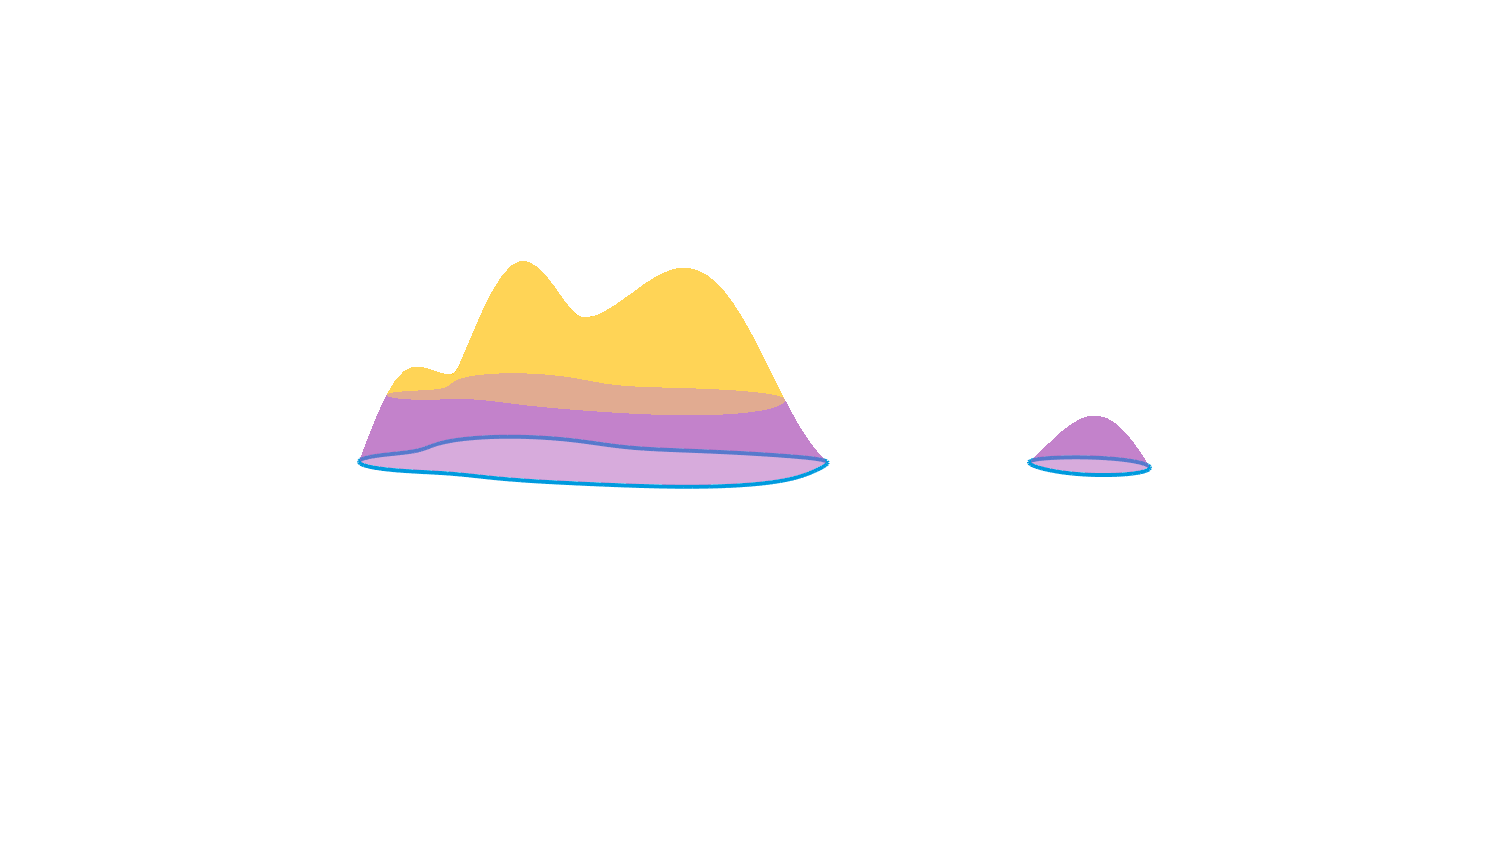
\includegraphics[trim=200 300 200 200, clip, width=0.3\textwidth]{scripts/figures/surf/ass1_C_side.png}
  
\includegraphics[trim=200 300 200 200, clip, width=0.3\textwidth]{scripts/figures/surf/ass1_D_side.png}
  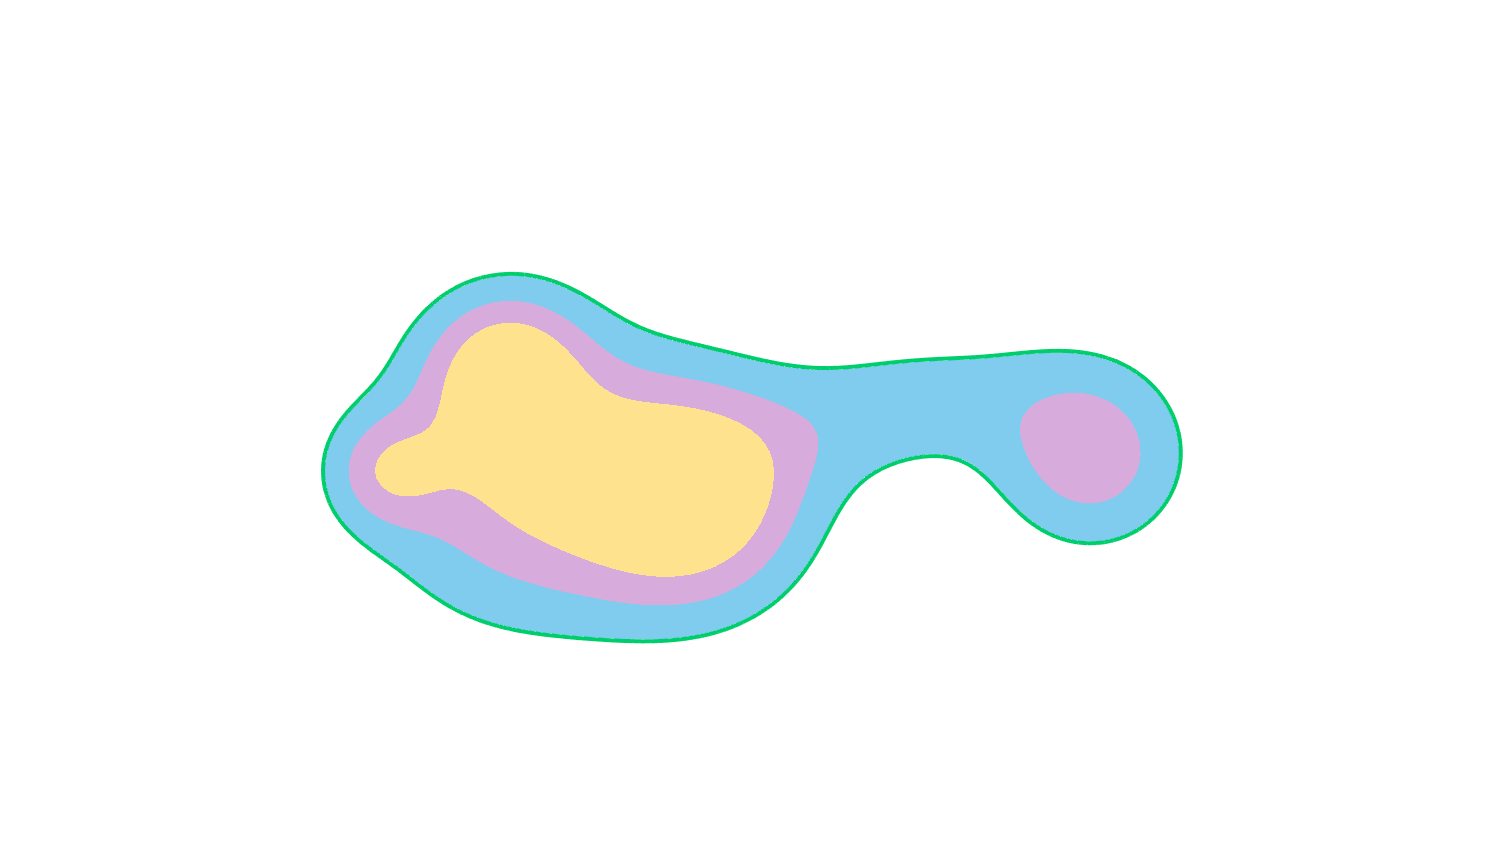
\includegraphics[trim=300 100 200 200, clip, width=0.3\textwidth]{scripts/figures/surf/ass2_B_top.png}
  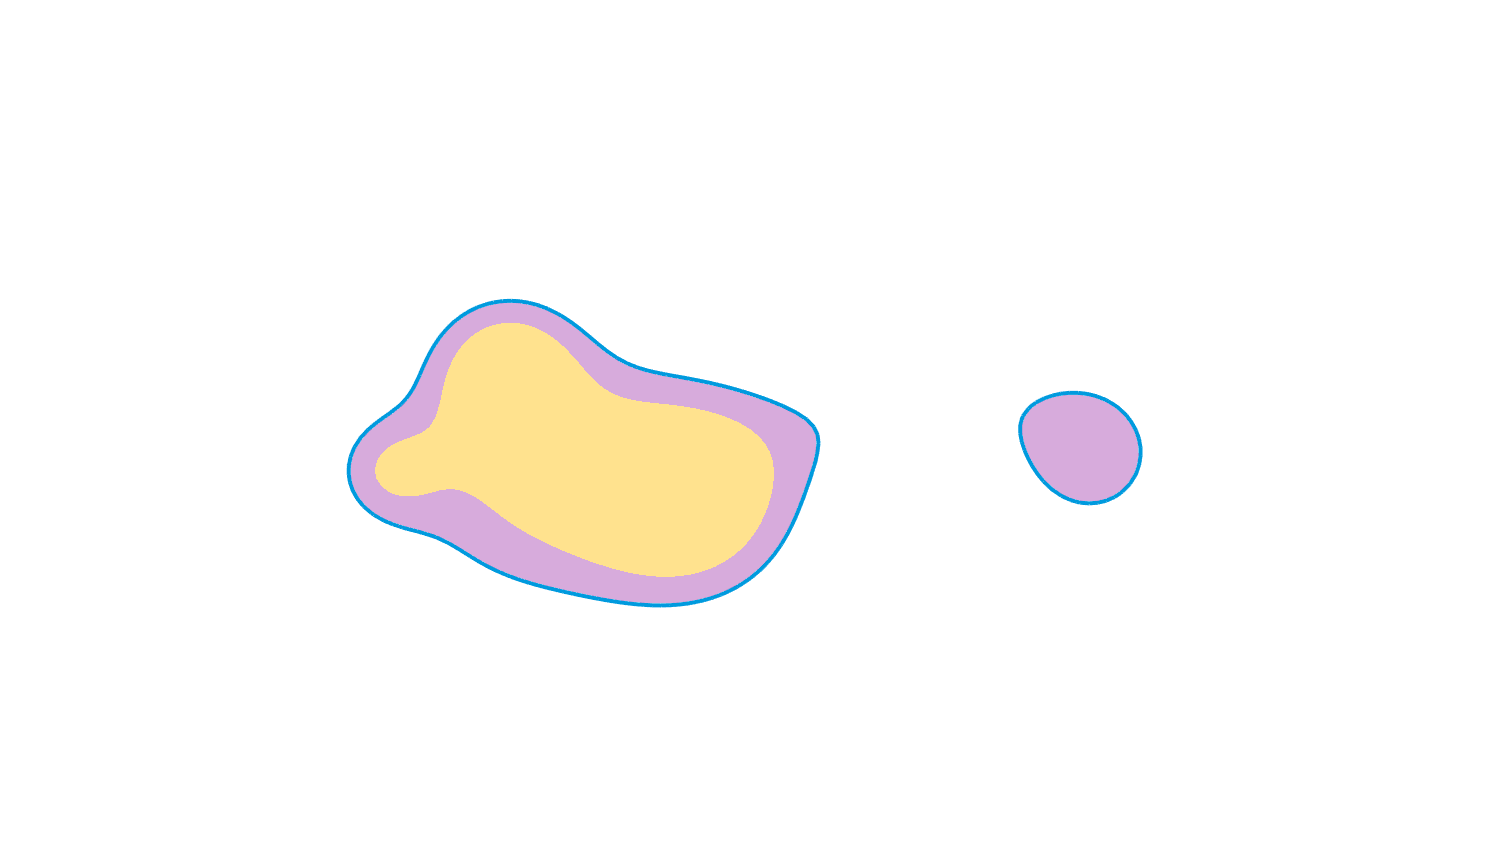
\includegraphics[trim=300 150 300 200, clip, width=0.3\textwidth]{scripts/figures/surf/ass1_C_top.png}
  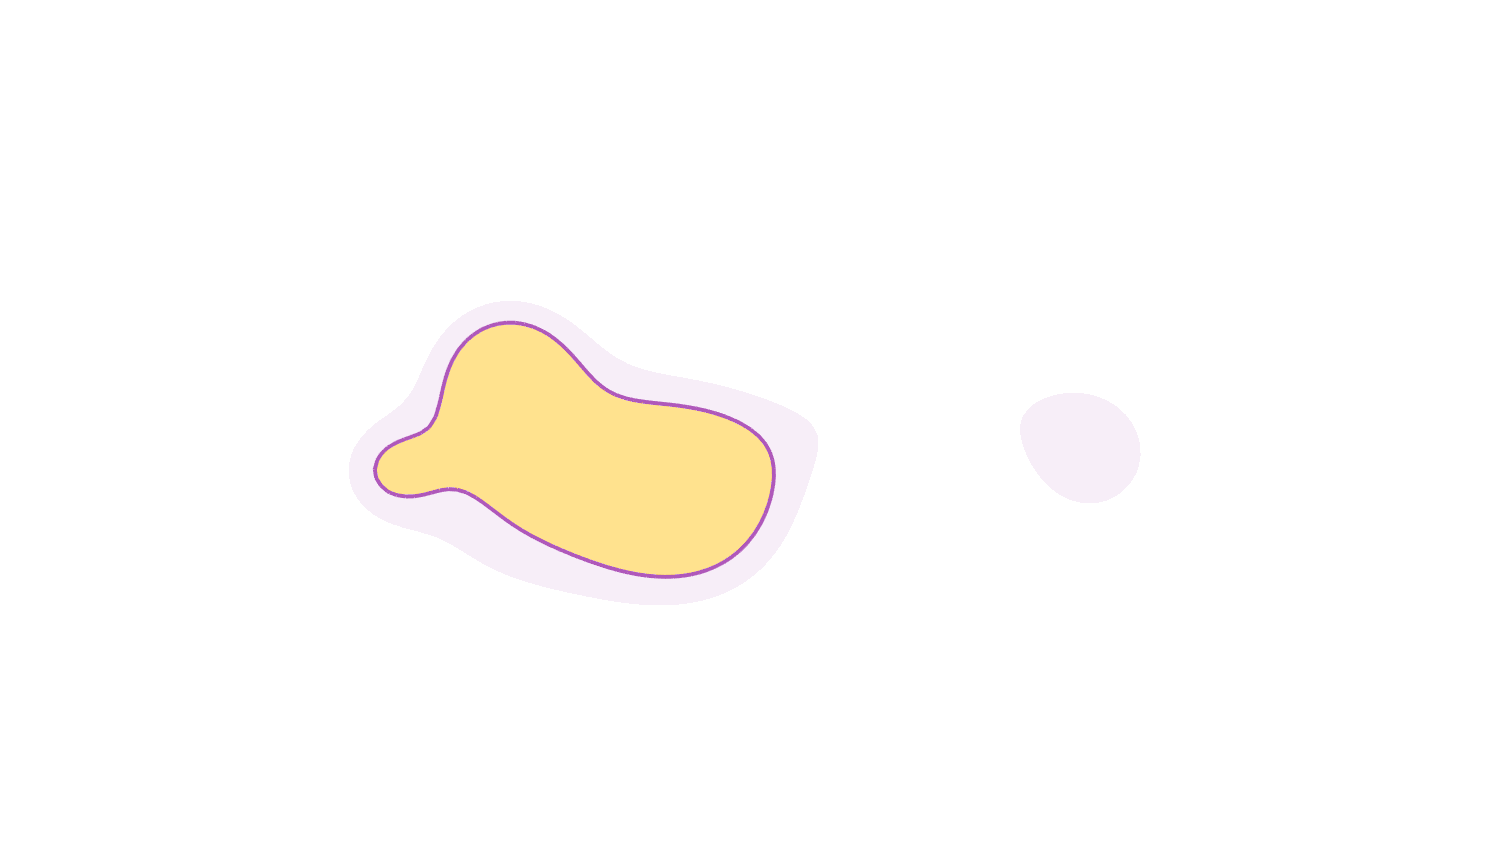
\includegraphics[trim=300 150 300 200, clip, width=0.3\textwidth]{scripts/figures/surf/ass1_D_top.png}
  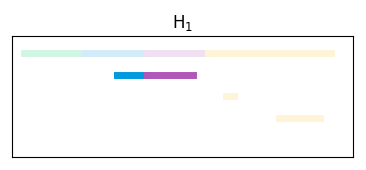
\includegraphics[width=0.5\textwidth]{scripts/figures/scalar_barcode_H1-masked.png}
  \caption{The blue level set does not satisfy either assumption as the smaller component is not in the inclusion from blue to green and it ``pinched out'' in the yellow region. This can be seen in the barcode shown as a feature that is born in the blue region and dies in the purple region.}
\end{figure}

% \begin{figure}[htbp]\label{fig:assumption2}
%   \centering
%   
\includegraphics[trim=200 300 200 200, clip, width=0.5\textwidth]{scripts/figures/surf/ass2_C_side.png}
%   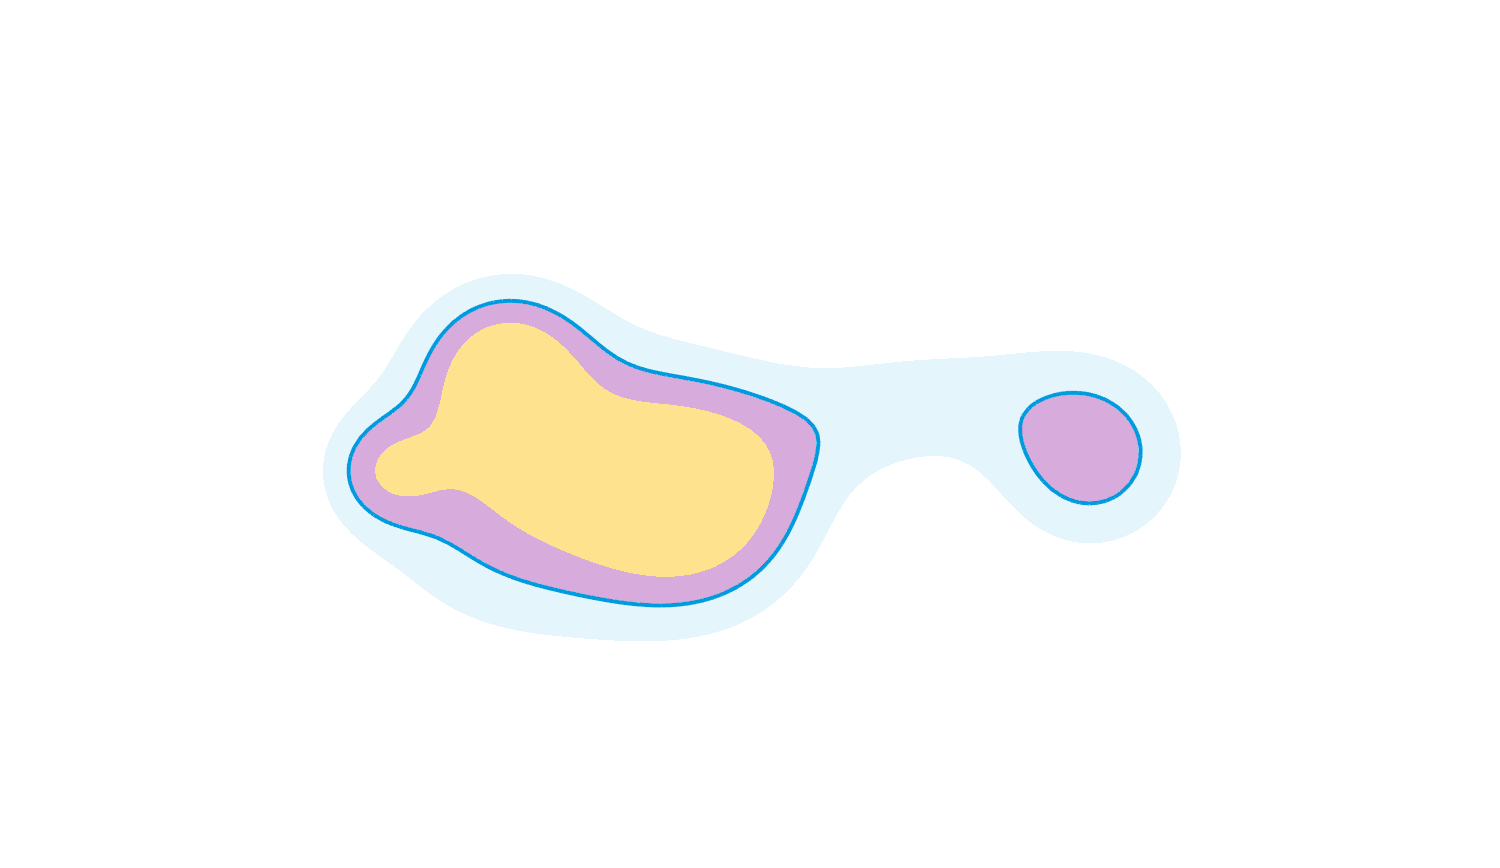
\includegraphics[trim=300 200 200 200, clip, width=0.3\textwidth]{scripts/figures/surf/ass2_C_top.png}
%   
\includegraphics[trim=200 300 200 200, clip, width=0.5\textwidth]{scripts/figures/surf/ass2_B_side.png}
%   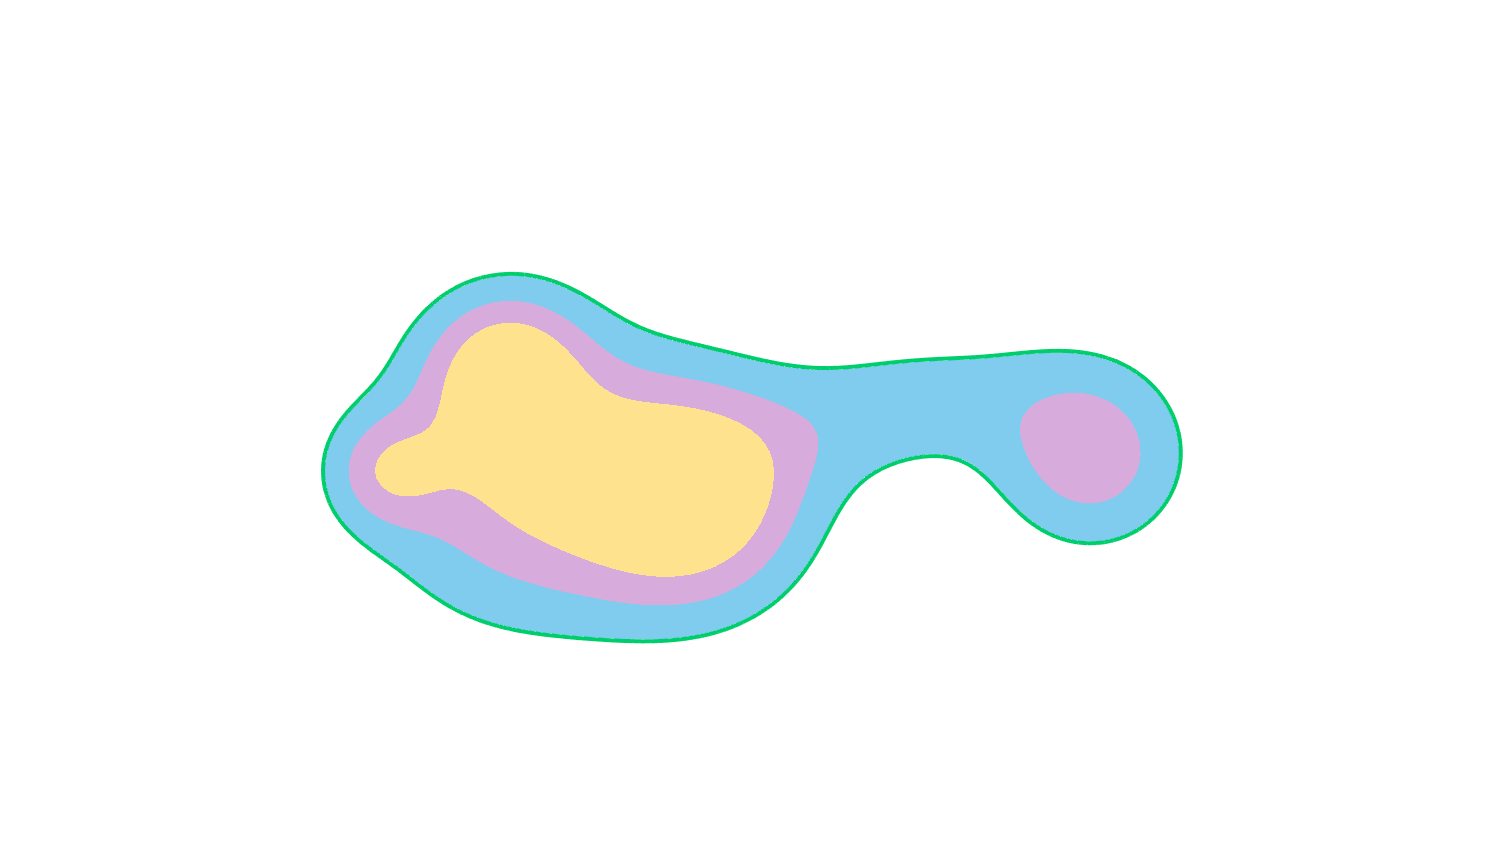
\includegraphics[trim=300 200 200 200, clip, width=0.3\textwidth]{scripts/figures/surf/ass2_B_top.png}
%   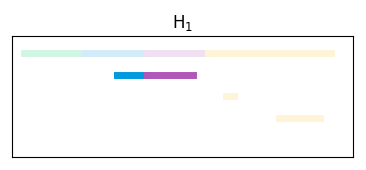
\includegraphics[scale=0.7]{scripts/figures/scalar_barcode_H1-masked.png}
%   \caption{\textbf{(Assumption 2)} The blue levelset does not satisfy Assumption 2 as the smaller component is not in the inclusion from blue to green.}
%           % This can be seen in the second feature of the barcode shown as a feature which is born in the blue region.}
% \end{figure}

\begin{lemma}\label{lem:assumption2}
  If $\hom_0(D\setminus B_\omega\hookrightarrow D\setminus B_{\omega+c(\delta+\zeta)})$ is injective and each component of $D\setminus B_\omega$ contains a point in $P$ then $\dim~\hom_0(\rips^\delta(P\setminus Q_{\omega-c\zeta})) \geq \dim~\hom_0(D\setminus B_\omega)$.
\end{lemma}

% The statement of Theorem~\ref{thm:geo_tcc} is in terms of the $0$-dimensional homology of complement spaces makes it difficult, if not impossible, to compute directly.
% The following lemma
The \fullversion details how to construct the following isomorphism using the Nerve Theorem along with Alexander Duality and the Universal Coefficient Theorem.
\[ \xi\N_w^{\e,k} : \hom_d(\cech^\e(P,Q_w))\to \hom_0(D\setminus Q_w^\e, D\setminus P^\e).\]
This isomorphism holds in the specific case when $P^\e\subseteq \intr_\X(D)$ and $D\setminus P^\e$, $D\setminus Q_w^\e$ are locally contractible.
We therefore provide the following definition for ease of exposition
\begin{definition}[$(\delta,\zeta,\omega)$-Sublevel Sample]
  For $\zeta\geq \delta > 0$, $\omega\in\R$, and a $c$-Lipschitz function $f: D\to \R$ a finite point set $P\subset D$ is said to be a \textbf{$(\delta, \zeta, \omega)$-sublevel sample} of $f$ if every component of $D\setminus B_\omega$ contains a point in $P$, $P^\delta\subset\intr_\X(D)$, and $D\setminus P^\delta$, $D\setminus Q_{\omega-c\zeta}^\delta$, and $D\setminus Q_{\omega+c\delta}^\delta$ are locally path connected in $\X$.
\end{definition}

\begin{theorem}[Algorithmic TCC]\label{thm:algo_tcc}
  Let $\X$ be an orientable $d$-manifold and let $D$ be a compact subset of $\X$.
  Let $f : D\to\R$ be $c$-Lipschitz function and $\omega\in\R$ and $\delta\leq\zeta < \varrho_D$ be constants such that $P\subset D$ is a $(\delta,\zeta,\omega)$-sublevel sample of $f$ and $B_{\omega - c(\zeta +\delta)}$ surrounds $D$ in $\X$.

  If $\hom_0(D\setminus B_{\omega+c(\delta+\zeta)}\hookrightarrow D\setminus B_\omega)$ is surjective, $\hom_0(D\setminus B_\omega\hookrightarrow D\setminus B_{\omega+c(\delta+\zeta)})$ is injective, and $\rk~\hom_d(\rips^\delta(P, Q_{\omega -c\zeta})\hookrightarrow \rips^{2\delta}(P, Q_{\omega+c\delta})) \geq \dim~\hom_0(\rips^\delta(P\setminus Q_{\omega-c\zeta}))$ then $D\setminus B_\omega\subseteq P^\delta$ and $Q_{\omega-c\zeta}^\delta$ surrounds $P^\delta$ in $D$.
\end{theorem}
\begin{proof}
  % We have the following commutative diagram
  % \[\begin{tikzcd}
  %   \hom_d(\cech^\delta(P, Q_{\omega-c\zeta})) \arrow{r}{q_{\cech}}\arrow{d}{\N_{\omega-c\zeta}^{\delta}} &
  %   \hom_d(\cech^\delta(P, Q_{\omega+c\delta})) \arrow{d}{\N_{\omega-c\zeta}^\delta}\\
  %   %
  %   \hom_d(P^\delta, Q_{\omega-c\zeta}^\delta))\arrow{r}{q} &
  %   \hom_d(P^\delta, Q_{\omega+c\delta}^\delta).
  % \end{tikzcd}\]
  % where vertical maps are isomorphisms provided by the Nerve Theorem and horizontal maps are induced by inclusions.

  Because $P$ is a $(\delta, \zeta, \omega)$-sublevel sample we have isomorphisms $\xi\N_{\omega-c\zeta}^\delta$ and $\xi\N_{\omega+c\delta}^\delta$ that commute with $q_{\cech}$ and $i : \hom_0(D\setminus Q_{\omega+c\delta}^\delta, D\setminus P^\delta)\to \hom_0(D\setminus Q_{\omega-c\zeta}^\delta, D\setminus P^\delta)$.
  Let $q_{\rips} : \hom_d(\rips^{\delta}(P, Q_{\omega-c\zeta}))\to\hom_d(\rips^{2\delta}(P, Q_{\omega+c\delta}))$ be induced by inclusion.
  Then $\rk~q_{\cech} \geq\rk~q_{\rips}$ as $q_{\rips}$ factors through $q_{\cech}$.
  As we have assumed $\hom_0(D\setminus B_\omega\hookrightarrow D\setminus B_{\omega-c(\delta+\zeta)})$ Lemma~\ref{lem:assumption2} implies $\dim~\hom_0(\rips^\delta(P\setminus Q_{\omega-c\zeta}))\geq \dim~\hom_0(D\setminus B_\omega)$.
  It follows that, whenever $\rk~q_{\rips} \geq \dim~\hom_0(\rips^\delta(P\setminus Q_{\omega-c\zeta}))$, we have
  \[ \rk~i = \rk~q_{\cech} \geq \rk~q_{\rips} \geq \dim~\hom_0(\rips^\delta(P\setminus Q_{\omega-c\zeta})) \geq \dim~\hom_0(D\setminus B_\omega).\]

  Because $j$ is surjective by hypothesis $\rk~j = \dim~\hom_0(\cmp{\B},\cmp{D}) = \dim~\hom_0(D\setminus B_\omega)$ so $\rk~j\geq \rk~i$ by Lemma~\ref{lem:psurj}.
  As we have shown $\rk~i\geq \dim~\hom_0(D\setminus B_\omega)$ it follows that $\rk~j = \rk~i$.
  Because $P$ is a finite point set we know that $\im~i$ is finite-dimensional and, because $\rk~i = \rk~j$, $\im~j=\hom_0(\cmp{\B}, \cmp{D})$ is finite dimensional as well.
  So $\im~j$ is isomorphic to $\im~i$ as a subspace of $\hom_0(\cmp{\Q^\of}, \cmp{P^\of})$ which, because $j$ is surjective, requires the map $\ell$ to be injective.
  Therefore $D\setminus\bb\subseteq P^\of$ and $\Q^\of$ surrounds $P^\of$ in $D$ by Lemma~\ref{lem:coverage}.
  %, Lemma~\ref{lem:cov_surrounds}.
  % As $j : \hom_0(D\setminus B_{\omega+c(\delta+\zeta)})\to \hom_0(D\setminus B_\omega)$ is surjective by assumption $\rk~j = \dim~\hom_0(D\setminus B_\omega)$, so $D\setminus B_\omega\subseteq P^\delta$ and $Q_{\omega-c\zeta}^\delta$ surrounds $P^\delta$ in $D$ by Theorem~\ref{thm:geo_tcc} as desired.
\end{proof}
